\documentclass[11pt,letterpaper,twoside]{article}
\usepackage[english]{babel}
\usepackage{amssymb,amsmath}
\usepackage{fancyhdr}
\usepackage{graphicx}
\usepackage{wrapfig}

 \oddsidemargin  0in \evensidemargin 0in
 \topmargin   -0.25in \headheight 0.25in \headsep 0.25in
 \textwidth   6.5in \textheight 8.75in \marginparsep 0pt \marginparwidth 0pt
 \parskip 1ex  \parindent 0ex \footskip 20pt

\newfont{\bssten}{cmssbx10}
\newfont{\bssnine}{cmssbx10 scaled 900}

%%%%%%%%%%%%%%%%%%%%%%%
\newcommand{\whatizit}{Lecture 17: Hypothesis Testing for Proportions}
%%%%%%%%%%%%%%%%%%%%%%%


\pagestyle{fancy}  
\fancyhead{\bssnine STOR 155,  \whatizit}
\fancyhead[RE]{} \fancyhead[LO]{}
\fancyhead[LE]{\bssnine \thepage} \fancyhead[RO]{\bssnine \thepage}
\lfoot{} \cfoot{} \rfoot{}   


\newcommand{\var}{\mathrm{Var}}



\begin{document}



\thispagestyle{empty} \vspace*{-0.75in}

{\bssten STOR 155: Introduction to Data Models and Inference \hfill June 14, 2024 \\
Prof. Will Lassiter  \hfill Page 1 of \pageref{totalpag}}
\vspace{10pt}
\begin{center} {{\Large \bf \whatizit}} \end{center}

Motivating example: My wife and I recently agreed to resolve all our petty disputes by rolling two dice she recently got from a friend and determining a winner based on their sum. She wins if 6, 7, 8, or 9 is rolled, and I win if 2, 3, 4, 5, 10, 11, or 12 is rolled. \vspace{6pt}

If these are fair dice, what is the probability that my wife wins our next dispute? \vspace{80pt}

So far we've had 72 disputes and my wife has won 52 of them.  Are these dice really fair? \vspace{200pt}

A {\bf hypothesis test} (or {\bf test of significance}) starts with ...

\begin{itemize}

\item \ \vspace{50pt}

\item \ \vspace{50pt}

\end{itemize}

and asks ...

\newpage

Terminology and notation: {\bf null hypothesis} and {\bf alternative hypothesis} \vspace{150pt}

Example: A social media app claims that in a poll of its American users, a healthy majority (55\%) approve of their personal data being collected and stored if it leads to better content recommendations from the app. A Pew Research survey asked 850 randomly chosen users if they are comfortable with personal data being collected in service of better recommendations, and only 46\% of respondents answered ``yes". Do these data provide convincing evidence that the proportion of American users who are comfortable with this data collection is less than 55\%? 

\begin{itemize}

\item Parameter of interest: \vspace{15pt}

\item Hypotheses: \vspace{15pt}

\end{itemize}

{\bf One-Sided z-Test for a Population Proportion} \vspace{200pt}

Back to example:

\newpage

Decision Errors

\begin{center}
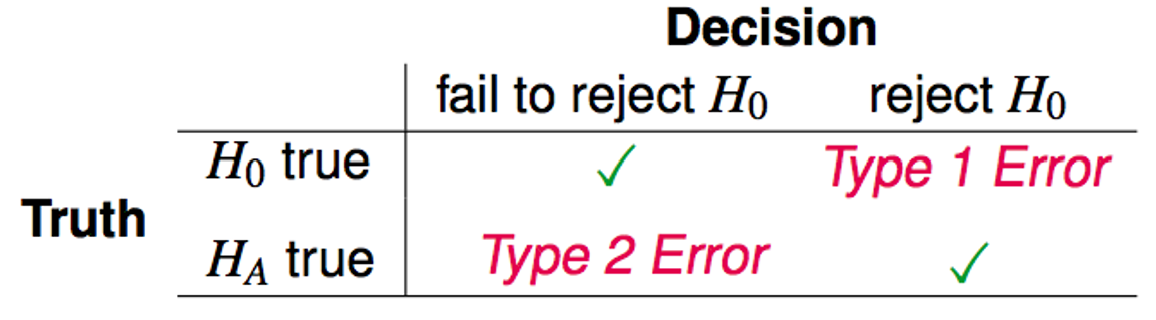
\includegraphics[scale=0.6]{errors.png}
\end{center}

Example: Criminal trial \vspace{120pt}

Example: In a SRS of 800 voters, 419 have indicated they will vote for Yoshi, the Mario Party’s candidate, for mayor.  Is it reasonable to conclude that a majority of voters favor Yoshi? \vspace{200pt}

What if we took another random sample of 800 voters and found that only 381 favored Yoshi? 


\newpage

{\bf Two-Sided z-Test for a Population Proportion} \vspace{250pt}

Example: $H_0: p = 0.46$  vs.  $H_A: p < 0.46$,  $z = -1.82$.  p-value? \vspace{50pt}
		
$H_0: p = 0.46$  vs.  $H_A: p \neq 0.46$,  $z = -1.82$.  p-value? \vspace{50pt}

Interpreting and using the p-value: {\bf statistical significance} 


\newpage


Typical language in published reports on statistical studies:

\begin{itemize}

\item ``The difference is statistically significant (P = 0.03)." \vspace{10pt}

\item ``The result is significantly greater than zero (z = 4.3, P < 0.0001)." \vspace{10pt}

\item ``The data do not support the conclusion that the rate has increased (z = 1.46, P = 0.1442)." \vspace{10pt}

\end{itemize}


Example: A drug that has been on the market for some time is known to produce a certain side effect in 42\% of patients. A new version of the drug is tested on 150 patients, and 51 of them develop the side effect.
We have no prior reason to believe that the new version of the drug has higher or lower incidence of the side effect; we only wonder whether this trial provides enough evidence to conclude that the new drug's incidence is different from 0.42.







\label{totalpag}
\end{document}
